\subsubsection{Prijava za teorijski ispit}
\label{subsubsec:prijava za ispit}
\begin{itemize}
  \item \textbf{Kratak opis}: Kandidat nakon zavrsenog pohadjanja casova teorije podnosi prijavu za polaganje teorijskog ispita
  \item \textbf{Učesnici}:
    \begin{itemize}
    \item Kandidat korisnik sistema koji se prijavljuje za ispit
    \end{itemize}
  \item \textbf{Preduslovi}:
    \begin{itemize}
    \item  Kandidat mora biti upisan u auto skolu.
    \item  Kandidat je zavrsio-odslusao sve casove terojie.
    \item  Kandidat je izmirio prethodne troskove prijave.
    \item  Kandidat je ulogovan na sistem.
    \item  Sistem je dosutpan.
    \item  Kandidat ima pristup internetu.
    \end{itemize}
  \item \textbf{Postuslovi}:
      \begin{itemize}
      \item Kandidat je podneo prijavu za polaganje teorijskog ispita.
      \end{itemize}
  \item \textbf{Osnovni tok}:
      \begin{enumerate}
        \item Kandidat otvara stranicu za prijavu polaganja teorijskog ispita.
        \item Sistem prikazuje formular za prijavljivanje teorijskog ispita.
        \item Kandidata popunjava formular.
        \item Kandidat potvrdjuje prijavu klikom na dugme.
        \item Sistem evidnetira prijavu.
        \item Sistem salje mail kandidatu o uspesnoj prijavi.  
      \end{enumerate}

  \item \textbf{Alternativni tokovi}:
      \begin{itemize}
        \item A1. \textbf{Neuspela validacija.}
        Ukoliku u koraku 3 sistem pronalazi neispravno polje formulara sistem obelezava polje koje treba ispraviti crvenom bojom, a ispod polja pise  uzrok neispravnosti. Nakon ponovnog ispravnog unosa podataka proces se nastavlja u korakku 5.
      \end{itemize}
      
  \item \textbf{Dodatne informacije}:
      \begin{itemize}
        \item Polja formulara za prijavu: Ime, Prezime, JMBG, Datum poslednjeg casa, Predavac, Skenirana licna karata 
      \end{itemize}
\end{itemize}

\begin{figure}[H]
  \begin{center}
      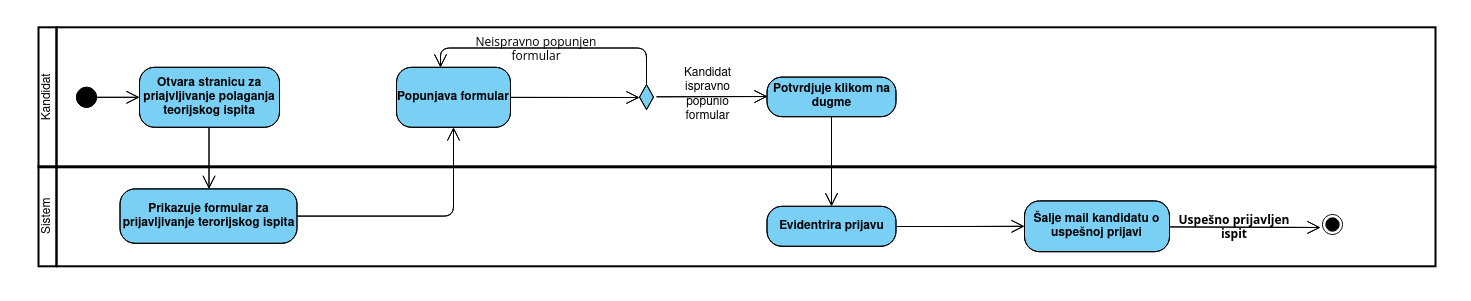
\includegraphics[width=140mm, height=70mm]{Diagrams/prijava za polaganje teorijskog ispita.png}
  \end{center}
  \caption {Dijagram aktivnosti - prijava za teorijski ispit}
  \label{activity_prijava_za_teoriju}

\end{figure}
